\documentclass[10 pt]{article}

\usepackage[top= 30mm, bottom=30mm, left=35mm, right=35mm]{geometry}
\usepackage[OT2]{fontenc}
\usepackage[serbian]{babel}
\usepackage{hyperref}
\usepackage{graphicx}
\usepackage{float}
\usepackage{caption}
\usepackage{enumitem}

\hypersetup{
	colorlinks=true,
	linktoc=all,
	linkcolor=blue,
}

\begin{document}
	
	\begin{titlepage} 
		\centering 
		
		\rule{\textwidth}{1pt}
		
		\vspace{2pt}\vspace{-\baselineskip} 
		
		\rule{\textwidth}{0.5pt}
		
		\vspace{0.025\textheight}
		
		{\Huge Informacioni sistem za iznoshenje smec1a}\\
		
		\vspace{0.020\textheight}
		
		\rule{0.5\textwidth}{1pt}
		
		\vspace{0.020\textheight}
		
		{\LARGE Grpuni projektni rad}
		
		\vspace{0.5\textheight}
		
		\begin{minipage}{0.4\textwidth}
			\begin{flushleft} \large
				\emph{Autori:}\\
				Nemanja Antic1\\
				Filip Lazic1\\
				Miroslav Mishljenovic1\\
				Marija Mijailovic1
			\end{flushleft}
		\end{minipage}
		~
		\begin{minipage}{0.5\textwidth}
			\begin{flushright} \large
				\emph{Predmet:}\\ 
				Informacioni sistemi\\
				\emph{Profesor:}\\ 
				Sasha Malkov\\
				\emph{Asistent:}\\ 
				Aleksandra Kocic1
			\end{flushright}
		\end{minipage}\\[2cm]
		
		{\large \today}\\[2cm]
		
		
	\end{titlepage}
	
	
	\thispagestyle{empty}
	
	\newpage
	\renewcommand*\contentsname{Sadrzhaj:}
	\tableofcontents
	
	\newpage

	%%%%%%%%%%%%%%%%%%%%%%%%%%%%%%%%%%%%%%%%%%%%%%%%%%%%%%%%%
	%						UVOD			 				%
	%%%%%%%%%%%%%%%%%%%%%%%%%%%%%%%%%%%%%%%%%%%%%%%%%%%%%%%%%
		
	\section{Uvod}
	
	Rad predstavlja predlog informacionog sistema za sluzhbu iznoshenja smec1a. Rad je radjen kao projekat iz predmeta "Informacioni sistemi" na Matematichkom fakultetu. Informacioni sistem bi trebao da zadovolji sve glavne potrebe i reshi probleme danashnjih sluzhbi iznoshenja smec1a. Pruzhanje relevantnih informacija o postojec1em sistemu u sluzhbi iznoshenja smec1a nam je pruzhio M.A., shef sluzhbe iznoshenja smec1a u  JKP-u ''Chistoc1a'' iz Smedereva.
	
	\subsection{Kratak opis sistema}
	
	Da bismo lakshe opisali sistem prvo c1emo navesti principe po kojima funkcionishe sluzhba za iznoshenje smec1a. Osnovni cilj je iznoshenje otpada sa raznih lokacija i njihovo pravilno odlaganje ili skladishtenje na za tu vrstu otpada predvidjen nachin.
	
	Klijenti mogu slati zahteve za iznoshenjem otpada. Sluzhba je duzhna da procesuira zahtev i pokusha da na shto efikasniji nachin obavi klijentove zahteve. Sluzhba se susrec1e sa raznim poteshkoc1ama kao shto su ogranichen broj radne snage i sredstava potrebnih za obavljanje posla. Sluzhba iznosi razlichite vrste otpada kao shto su reciklazhni, kabasti, elektrichni, hemijski, medicinski itd.
	
	Za svaku vrstu otpada postoji posebna procedura koja se mora isposhtovati, od specijalne opreme za tu vrstu otpada, preko nachina na koji se prevozi, do krajnje lokacije gde se otpad odlazhe ili skladishti(razne vrste deponija, magacini i sl.).
	
	Sistem pruzha podrshku zaposlenima da lakshe, brzhe i efikasnije obavljaju svoje poslove. Takodje sistem olakshava i komunikaciju sa klijentima (preko onlajn formulara ili telefonskog poziva). U sluzhbi je svako odgovoran za svoj deo posla, nema preklapanja. Sistem c1e pruzhiti svakom zaposlenom samo skup funkcionalnosti koje su predvidjene za njegovu radnu poziciju. U bazi se chuvaju podaci o svim zaposlenima i njihovim obavljenim poslovima.
	
	\subsection{Uchesnici u sistemu}
	
	\begin{itemize}
		
		\item\textbf{\textit{Upravnik}} - rukovodi poslovanjem sluzhbe. Upravniku sistem nudi uvid u rad zaposlenih u firmi. Pruzha mu moguc1nost da smenjuje radnike, zaposhljava, daje otkaze, dopushta odmore.
		
		\item\textbf{\textit{Dispecher}} - zaduzhen je za komunikaciju sa klijentom. Prihvata zahteve klijenata i prosledjuje poslove koordinatorima. Zahtevi klijenata se prikupljaju i chuvaju u sistemu dok ih dispecher ne obradi.
		
		\item\textbf{\textit{Klijent}} - shalje zahteve za obavljanjem posla. Sistem mu omoguc1ava da preko onlajn formulara poshalje zahtev. Takodje klijent mozhe i direktno kontaktirati dispechera preko telefona pri chemu zajedno definishu zahtev. 
		
		\item\textbf{\textit{Koordinator}} - vrshi ulogu operativca. Njegov glavni zadatak je da organizuje poslove iznoshenja otpada. Koordinator ima moguc1nosti da izabere slobodne radnike, vozache, vozila i ostala sredstva koja su mu na raspolaganju da obavi posao. Duzhnost koordinatira je da evidentira da li je posao zavrshen do kraja i ako nije da navede razlog. Ovaj razlog mozhe da vidi dispecher pri chemu treba da obavesti klijenta ako njegov zahtev nije ispunjen.
		
		\item\textbf{\textit{Radnik}} - ima zadatak da radi po nalogu. Njegova obaveza je da izvrshi zadatak i obavesti koordinatora da je posao uradjen i ako nije, da slusha dalja uput{s}tva koordinatora.
		
		\item\textbf{\textit{Vozach}} - po nalogu dobija posao, tachnu rutu na koju mora da ode. Vozach je rasporedjen na neko vozilo i na njemu obavlja svoj deo posla.
		
		\item\textbf{\textit{Magacioner}} - njegov zadatak je da uredjaje koji su stigli do magacina, smesti u magacin i unese u bazu.
		
		\item\textbf{\textit{Menad2er prodaje}} - njegov zadatak je da izlazi na teren i procenjuje otpad koji se mozhe otkupiti i preprodati.
		Njega angazhuje dispecher. Duzhnost menad2era je da odgovori na zahtev klijenta da li je zahtev prihvac1en kao i cenu otpada, ako je odgovor potvrdan. Takodje menad2er prodaje odredjuje cenu uredjaja iz magacin i stavlja ih na aukciju.
	
	\end{itemize}	
	
	
	\section{Analiza sistema}
	
	Analizirali smo postojec1i sistem JKP ''Chistoc1a''. Trenutni sistem funkcionishe jako loshe. Sistem je zastareo i ne koristi u potpunosti prednosti koje nam nude informacione tehnologije. Vec1ina informacija i podataka nalazi se na papirima. Poslovi su vrlo neprecizno raspodeljeni medju zaposlenima. Na primer, u trenutnom sistemu nije jasno definisano ko je zaduzhen za saradnju sa klijentima, pa se deshava da klijenti pozivaju operativce (koordinatore) da im reshe konkretan problem. Koordinatori u tom sluchaju budu prebukirani i ne mogu da vrshe posao efikasno. Takodje, efikasnost je smanjena samim tim shto se podaci o zaposlenima i druge chesto upotrebljivane informacije chuvaju u vidu Eksel tabela. Samim tim menjanje podataka je vrlo sporo i nebezbedno. Ne postoji nikakav interfejs preko koga bi se moglo lakshe, brzhe i bezbednije menjati podaci. Dobra stvar u trenutnom sistemu je podsistem koji prati vozila na terenu. Sistem je nov, pouzdan i zaista mnogo doprinosi koordinatorima da  vrlo lako procenjuju vreme trajanja nekog posla, kashnjenje, radnu snagu potrebnu za neki posao, i sl. U svakom trenutku koordinator mozhe da proveri geografski u kom delu grada se nalaze ljudi koji iznose otpad, koliko su se dugo zadrzhali i sl.
	
	Nov sistem bi trebao da omoguc1i pre svega bolju komunikaciju izmedju zaposlenih, kao i lakshu evidenciju poslova, zadataka, zahteva i drugih bitnih poslova. Sistem c1e koristiti informacione tehnologije (veb pretezhno) da omoguc1i brzhi i lakshi protok informacija. Podaci o zaposlenima, o trenutnim, zavrshenim i buduc1im poslovima, zahtevi klijenata, stanja vozila itd. c1e se nalaziti u bazi, a sistem bi trebao da omoguc1i brz i lak pristup podacima preko korisnichkih intefejsa. Takodje novim sistemom bi bila jasna podela zaduzhenja u sluzhbi. Odnosi sa klijentima se jasno dekomponuju od samog procesa iznoshenja otpada. Prikaz informacionog sistema je dat na slikama \ref{fig:dijagramKonteksta} i \ref{fig:dijagramTokaPodataka}
	
	\begin{figure}[H]
		\centering
		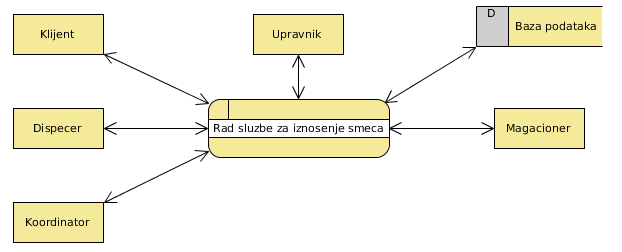
\includegraphics[width=15cm,height=15cm,keepaspectratio]{slike/DijagramKonteksta.png}\\
		\caption{Dijagram konteksta}
		\label{fig:dijagramKonteksta}
	\end{figure}

	\begin{figure}[H]
		\centering
		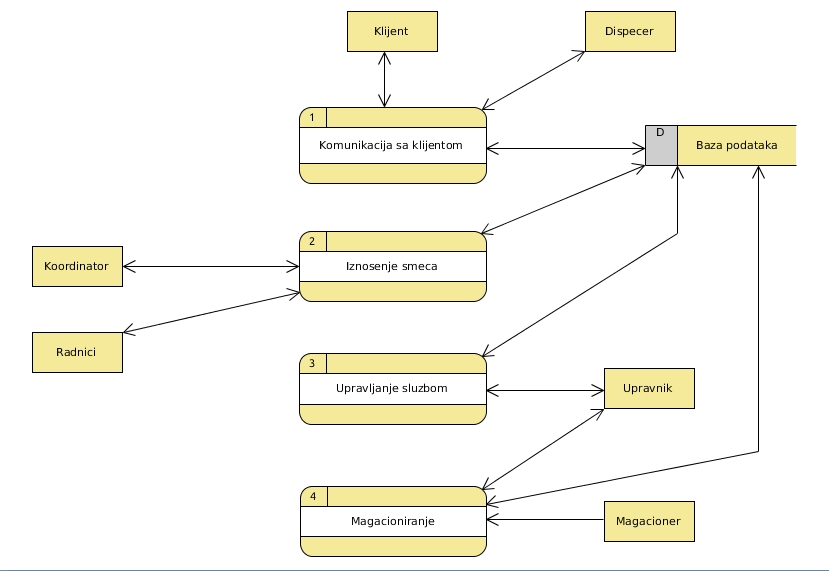
\includegraphics[width=15cm,height=15cm,keepaspectratio]{slike/DTP.png}\\
		\caption{Dijagram toka podataka}
		\label{fig:dijagramTokaPodataka}
	\end{figure}
	
	
	%%%%%%%%%%%%%%%%%%%%%%%%%%%%%%%%%%%%%%%%%%%%%%%%%%%%%%%%%
	%				SLUCAJEVI UPOTREBE		 				%
	%%%%%%%%%%%%%%%%%%%%%%%%%%%%%%%%%%%%%%%%%%%%%%%%%%%%%%%%%
	
	\section{Sluchajevi upotrebe}
	
	\subsection{Definisanje zahteva}
	
	\begin{figure}[H]
		\centering
		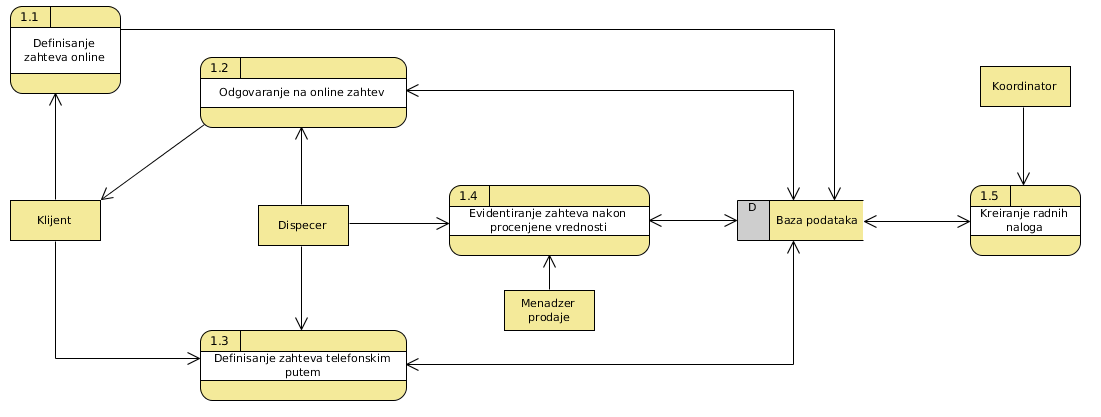
\includegraphics[width=15cm,height=15cm,keepaspectratio]{slike/DTPDefinisanjeZahteva.png}\\
		\caption{Dijagram toka podataka za definisanje zahteva}
	\end{figure}
	
	\subsubsection{Sluchaj upotrebe - Definisanje zahteva onlajn}
	
		\begin{itemize}
			
			\item\textit{Kratak opis} - Klijent kontaktira sluzhbu tako shto popunjava onlajn formular.
	
			\item\textit{Akter} - Klijent - shalje zahtev za iznoshenjem otpada popunjavanjem formulara.
			
			\item\textit{Preduslov} - Internet konekcija je stabilna, sajt je ispravan.
			
			\item\textit{Postuslov} - Zahtev klijenta je uspeshno poslat.

			
			\item\textit{Osnovni tok} 
				\begin{enumerate}
					\item Klijent pristupa sajtu sluzhbe.

					\item Klijent popunjava formular.

					\item Klijent potvrdjuje zheljenu uslugu klikom na "poshalji".
				\end{enumerate}
			
			\item\textit{Dodatne informacije}
- Formular sadrzhi sledec1e informacije : ime, prezime, adresu, broj telefona, imejl, lokaciju otpada, kratak opis shta klijent tachno zahteva, vrstu otpada, datum kada zheli da se otpad iznese.
			

		\end{itemize}
	
	\subsubsection{Sluchaj upotrebe - Odgovaranje na onlajn zahtev}
	
		\begin{itemize}
			\item\textit{Kratak opis} - Dispecher u toku radnog vremena proverava pristigle zahteve, odogovara na njih i evidentira ih u sistem.
			
			\item\textit{Akter} - Dispecher - prima zahtev klijenta, evidentria ga i odgovara na njega.
			
			\item\textit{Preduslovi}
				\begin{enumerate}
					\item Klijent je poslao zahtev.
					\item Dispecher je na svom radnom mestu(u bazi ima status aktivan).
					\item Baza je ispravna.
				\end{enumerate} 
			
			\item\textit{Postuslov} - Dispecher je uspeshno evidentirao zahtev klijenta u bazu podataka.
			
			\item\textit{Osnovni tok}
				\begin{enumerate}
					\item Dispecher pristupa delu informacionog sistema za proveru novih zahteva.
					\item Dispecher proverava pristigli zahtev.
					\item Dispecher upisuje podatke iz formulara u sistem.
					\item Sistem obaveshtava klijenta da je njegov zahtev uspeshno primljen.
				\end{enumerate}
			
			\item\textit{Podtok}
				\begin{enumerate}
					\item [4.] U sluchaju da se pristigli zahtev tiche iznoshenja elektrichnog otpada. Sistem obaveshtava klijenta da c1e biti kontaktiran od strane menad2era prodaje.
				\end{enumerate}
			
			\item\textit{Alternativni tok}
				\begin{enumerate}
					\item [2.] Posao je nemoguc1e izvrshiti tog datuma kada je klijent zahtevao. - Obaveshtava se klijent i sluchaj upotrebe se ovde zavrshava.
				\end{enumerate}
		\end{itemize}
	
	\subsubsection{Sluchaj upotrebe - Definisanje zahteva telefonskim putem}
	
		\begin{itemize}
			
			\item\textit{Kratak opis} - Klijent kontaktira sluzhbu putem telefona.

			
			\item\textit{Akteri} 
				\begin{enumerate}
					\item Klijent - kreira zahtev tako shto kontaktira sluzhbu putem telefona.
					\item Dispecer - prima zahtev klijenta.
				\end{enumerate}

			
			\item\textit{Preduslovi} 
				\begin{enumerate}
					\item Klijent kontaktira sluzhbu u toku  radnog vremena.
					\item Dispecher je na svom radnom mestu(u bazi ima status aktivan).

					\item Baza je ispravna.

				\end{enumerate}
			
			\item\textit{Postuslovi} - Dispecher je uspeshno evidentirao zahtev klijenta u bazu podataka.

			
			\item\textit{Osnovni tok}

				\begin{enumerate}
					\item Klijent poziva sluzhbu.

					\item Klijent dispecheru saopshtava sve potrebne informacije u vezi sa zahtevom.

					\item Dispecher potvrdjuje zahtev.

					\item Dispecher upisuje podatke u sistem.

				\end{enumerate}
			
			\item\textit{Podtok}
				\begin{enumerate}
					\item [3.] U sluchaju da je zahtev klijenta za iznoshenje elektrichnog otpada. Dispecher obaveshtava klijenta da c1e biti kontaktiran od strane menad2era prodaje.
				\end{enumerate}
			
			\item\textit{Alternativni tok}
				\begin{enumerate}
					\item [3.] Posao je nemoguc1e izvrshiti tog datuma kada je klijent zahtevao.
- Obaveshtava se klijent i sluchaj upotrebe se vrac1a na korak 2.

					
				\end{enumerate}

			
			\item\textit{Dodatne informacije}
-	Klijent prilikom kontaktiranja navodi sledec1e informacije :
ime, prezime, adresu, broj telefona, imejl, lokaciju otpada, kratak opis shta klijent tachno zahteva, vrstu otpada, datum kada zheli da se otpad iznese.

			
		\end{itemize}
	
	\subsubsection{Sluchaj upotrebe - Evidentiranje zahteva nakon procenjene vrednosti}
	
		\begin{itemize}

			\item\textit{Kratak opis} - Prilikom zahteva koji se tiche iznoshenja elektrichnog otpada, na teren se prvo shalje menad2er prodaje,
			kako bi procenio vrednost uredjaja. Uredjaji koji se procenjuju su:
			laptopovi, desktop rachunari, shtampachi, skeneri, televizori, telefoni, konzole za video igre.
			
			\item\textit{Akteri}
				\begin{enumerate}
					\item Menad2er prodaje - izlazi na teren radi procenjivanja novchane vrednosti uredjaja i dopunjuje zahtev klijenta.
					\item Dispecher - obaveshtava menad2era prodaje o izlasku na teren.
				\end{enumerate}
			
			\item\textit{Preduslovi} 
				\begin{enumerate} 
					\item Prilikom definisanja zahteva, klijent je obaveshten o izlasku menad2era prodaje na teren.
					\item Dispecher je uspeshno zabelezhio zahtev klijenta.
					\item Menad2er prodaje je na svom radnom mestu.
					\item Menad2er prodaje je obuchen za posao procenitelja.
				\end{enumerate}			
			
			\item\textit{Postuslovi}
				\begin{enumerate}
					\item Definisan je zahtev korisnika. 
					\item Dodata je cena otkupa.
					\item Zahtev je evidentiran u bazi.
				\end{enumerate}
			
			\item\textit{Osnovni tok}
				\begin{enumerate} 
					\item Dispecher obaveshtava menad2era prodaje da je stigao zahtev za iznoshenje elektrichnog otpada.
					\item Menad2er prodaje izlazi na teren radi procene.
					\item Menad2er prodaje vrshi procenu.
					\item Menad2er prodaje dopunjuje zahtev korisnika tako shto dodaje cenu usluge.
				\end{enumerate}
			
			\item\textit{Alternativni tok}
				\begin{enumerate}
					\item [4.] U sluchaju da su pregovori zavrsheni negativno, menad2er prodaje brishe zahtev iz baze. - Sluchaj upotrebe se ovde zavrshava.
				\end{enumerate}
			
		\end{itemize}
	
	
	\subsubsection{Sluchaj upotrebe - Kreiranje radnih naloga}
	
		\begin{itemize}
		
			\item\textit{Kratak opis} - Koordinator na osnovu raspolozhivih radnika i vozila kreira radne naloge.
			
			\item\textit{Akter} - Koordinator - zaduzhen je za kreiranje i shtampanje radnih naloga.
			
			\item\textit{Preduslovi}
				\begin{enumerate}
					\item Zahtev je ispravno definisan i evidentiran u bazi.
					\item Radnici i vozila su raspolozhivi.
				\end{enumerate}
			
			\item\textit{Postuslov} - Radni nalozi su kreirani i uneti u bazu.
			
			\item\textit{Osnovni tok}
				\begin{enumerate}
					\item Koordinator se konektuje na bazu.
					\item Koordniator na osnovu raspolozhivog stanja sastavlja radne naloge.
					\item Koordinator shtampa radne naloge.
				\end{enumerate}
			
		\end{itemize}
	
	%----------------------------------------------------------------
	
	\subsection{Upravljanje sluzhbom}
	
	\begin{figure}[H]
		\centering
		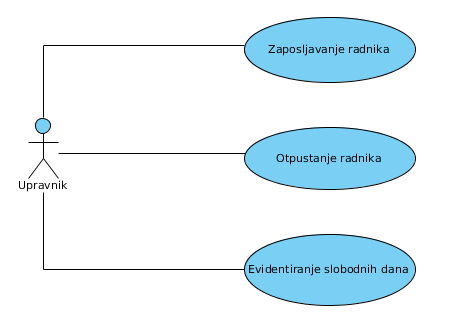
\includegraphics[width=12cm,height=12cm,keepaspectratio]{slike/UCUpravljanjeSluzbom.png}\\
		\caption{Dijagram upravljanja sluzhbom}
	\end{figure}
	
	\subsubsection{Sluchaj uptorebe - Zaposhljavanje radnika}
		
		\begin{itemize}
			\item\textit{Akter} - Upravnik vrshi unos zaposlenog u bazu.

			
			\item\textit{Preduslov} - Upravnik ima sve potrebne informacije o zaposlenom.

			
			\item\textit{Postuslov} - Novi zaposleni je dodat u sistem.

			
			\item\textit{Osnovni tok}
				\begin{enumerate}
					\item Upravnik pristupa delu sistema za unos podataka o zaposlenima.

					\item Upravnik bira vrstu zaposlenog (koordinator, magacioner, dispecher, radnik, vozach, menad2er prodaje).

					\item Upravnik unosi sve potrebne informacije o zaposlenom.

					\item Upravnik zavrshava unos klikom na opciju ''dodaj''.

					\item Sistem obaveshtava upravnika o uspeshnom dodavanju novog zaposlenog.

				\end{enumerate}
			
			\item\textit{Alternativni tok}
				\begin{enumerate}
					\item [3.] Upravnik je uvideo nepravilnosti u prikupljenim podacima. U tom sluchaju upravnik kontaktira zaposlenog kako bi dobio ispravne podatke.
- Sluchaj upotrebe se nastavlja od koraka 2.

					\item [5.] Sistem obaveshtava upravnika  da radnik nije uspeshno dodat. - Sluchaj upotrebe se nastavlja  od koraka 2.

				\end{enumerate}
				
			\item\textit{Dodatne informacije} - Neophodni uslovi za unos novog zaposlenog : id(jmbg), ime, prezime, datum zaposhljenja, vrsta posla koju obavlja, broj radnih dana, broj slobodnih dana, plata.

			
		\end{itemize}
	
	\subsubsection{Sluchaj upotrebe - Otpushtanje radnika}
		
		\begin{itemize}
			\item\textit{Akter} - Upravnik vrshi brisanje zaposlenog iz baze.
			
			\item\textit{Preduslov} - Upravnik ima sve potrebne informacije o zaposlenom kog zheli da otpusti.

			
			\item\textit{Postuslov} - Zaposleni je izbrisan iz sistema.

			
			\item\textit{Osnovni tok}
				\begin{enumerate}
					\item Upravnik pristupa delu sistema za pruzhanje informacija o zaposlenima.

					\item Upravnik pronalazi zaposlenog kog zheli da otupusti.

					\item Upravnik selektuje zaposlenog i klikom na opciju	''izbrishi'' brishe zaposlenog iz sistema.

					\item Sistem obaveshtava upravnika o uspeshnom brisanju bivsheg zaposlenog.

				\end{enumerate}
			
			\item\textit{Alternativni tok}
				\begin{enumerate}
					\item [4.] Sistem obaveshtava upravnika da radnik nije uspeshno obrisan. - Sluchaj upotrebe se nastavlja  od koraka 2.

				\end{enumerate}
			
		\end{itemize}
		
		
	\subsubsection{Sluchaj upotrebe - Evidentiranje slobodnih dana}
	
		\begin{itemize}
			
			\item\textit{Kratak opis} - Upravnik pregleda zahteve zaposlenih za slobodnim danima i procenjuje da li c1e zahtev prihvatiti. 

				
			\item\textit{Akter} - Upravnik vrshi evidenciju slobodnih dana zaposlenih.

			
			\item\textit{Preduslov} - Zaposleni ima dovoljno slobodnih dana.

			
			\item\textit{Postuslov} - U sistemu je evidentiran zahtev zaposlenog.

			
			\item\textit{Osnovni tok}
				\begin{enumerate}
					\item Upravnik dobija zahteve zaposlenog. 

					\item Upravnik pristupa delu sistema za pruzhanje informacija o zaposlenima.

					\item Upravnik razmatra zahteve zaposlenog.

					\item Upravnik unosi u sistem potrebne informacije.

					\item Sistem obaveshtava upravnika da je zahtev uspeshno obradjen.

				\end{enumerate}
			
			\item\textit{Alternativni tok}
				\begin{enumerate}
					\item [3.] Upravnik nije u moguc1nosti da dozvoli zaposlenom slobodne dane u skladu sa zahtevima zaposlenog.
- Sluchaj upotrebe se nastavlja od koraka 1.

					\item [5.] Sistem obaveshtava upravnika da zahtev nije uspeshno obradjen. - Sluchaj upotrebe se nastavlja od koraka 4.
			
				\end{enumerate}
			
			\item\textit{Dodatne informacije} - U zahtevu koji shalje zaposleni se nalazhe datum pochetka i datum kraja odmora. Opciono, zaposleni mozhe u zahtevu napisati i razlog.

			
		\end{itemize}
		
	%----------------------------------------------------------------
	
	\subsection{Iznoshenje otpada}
	
	\begin{figure}[H]
		\centering
		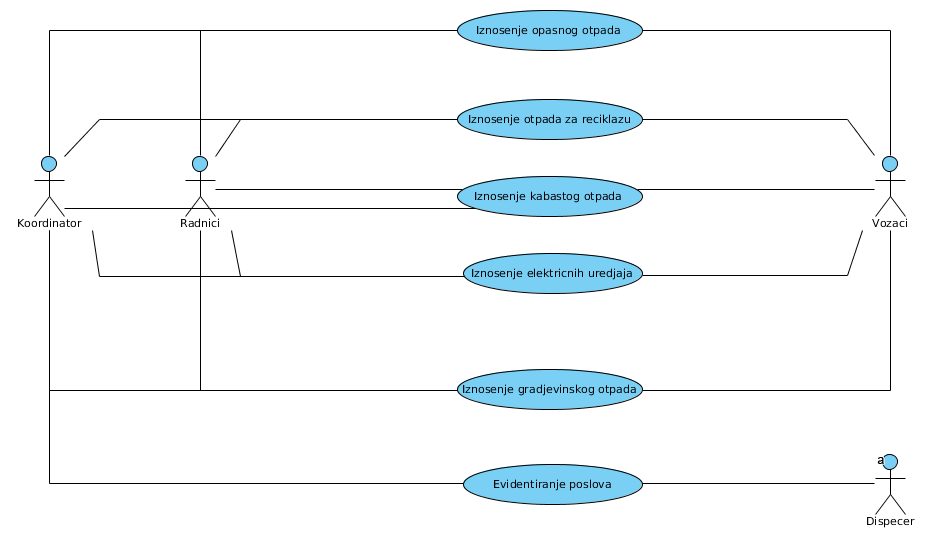
\includegraphics[width=15cm,height=15cm,keepaspectratio]{slike/UCIznosenjeSmeca.png}\\
		\caption{Dijagram iznoshenja otpada}
	\end{figure}
	
	\textbf{Opis osnovnog sluchaja upotrebe iznoshenja otpada}\\
		
	Iznoshenje otpada je proces koji se u zavisnosti od vrste otpada razlichito realizuje.
	Opisac1emo elemente koji su zajednichki za sve sluchajeve upotrebe.
	U sluchajevima upotrebe na nizhem nivou, bic1e razjashnjene specificnosti
	pojedinih sluchajeva upotrebe i dodatno objashnjene stavke koje to zahtevaju.
	
	\begin{itemize}
		\label{OsnovniSlucaj}
		\item\textit{Akteri}
			\begin{enumerate}
				\item Koordinator - predaje radni nalog radnicima, uz eventualna dodatna uput{s}tva.
				\item Radnici - izlaze na teren sa odgovarajuc1om opremom.
				\item Vozachi - osobe koja vrshe prevoz radnika i otpada.
			\end{enumerate}		
			
		\item\textit{Preduslovi}
			\begin{enumerate}
				\item Radni nalog je isrpavno definisan.
				\item Raspolozhiva je odgovarajuc1a oprema(kamion,odela,alat).
				\item Radnici su obucheni za rad sa odgovarajuc1om opremom.
				\item Radnici vrshe posao u skladu sa predvidjenim merama bezbednosti.
				\item Vozachi su doveli radnike na tachnu lokaciju.
				\item Vozachi imaju dozvolu za vozilo koje im je dato na upravljanje.
			\end{enumerate}
		
		\item\textit{Postuslovi}
			\begin{enumerate}
				\item Otpad je dostavljen na odgovarajuc1e mesto(deponija,magacin,reciklazhni centar,spaljivanje).
				\item Koordinator je obaveshten o is{h}odu posla.
			\end{enumerate}
		
		\item\textit{Osnovni tok}
			\begin{enumerate}
				\item Radnici preuzimaju nalog od koordinatora.
				\item Radnici dolaze na predvidjenu lokaciju.
				\item Radnici izvrshavaju iznoshenje.
				\item Radnici obaveshtavaju koordinatora o is{h}odu posla.(pozivom, SMS-om, imejl-om)
				\item Vozachi i radnici se vrac1aju kod koordinatora.
			\end{enumerate}
		
		\item\textit{Alternativni tok}
			\begin{enumerate}
				\item [2.] U sluchaju nemoguc1nosti dolaska na lokaciju, radnici obaveshtavaju koordinatora i vrac1aju se u firmu. Posao se odlazhe do daljnjeg. - Sluchaj upotrebe se nastavlja od koraka 4. 
			\end{enumerate}
			
	\end{itemize}		
	
	\subsubsection{Sluchaj upotrebe - Iznoshenje opasnog otpada}
		
		\begin{itemize}
			
			\item\textit{Kratak opis} - Sluzhba se bavi odnoshenjem opasnog otpada koji podrazumeva: 
				\begin{enumerate}
					\item[a)] hemikalije(zapaljive, nezapaljive),
					\item[b)] medicinski otpad (shpricevi, vate, zavoji, gips, infektivni otpad, lekovi kojima je istekao rok upotrebe itd),
					\item[v)] radioaktivni otpad (kontaminirani papir, vata, PVC, igle, oshtri metalni predmeti, razna zashtitna oprema, kontaminirani ili aktivirani metalni i plastichni delovi razlichitih oblika i dimenzija, techni radioaktivni otpad, suv i chvrst radioaktivni otpad koji se deli na  dve  podkategorije:
						otpad  koji  mozhe da se presuje i otpad koji ne mozhe da se presuje)
				\end{enumerate}
			
			
			\item\textit{Akteri}\\\\ 
				1. - 3. Isti kao u opisu osnovnog sluchaja \ref{OsnovniSlucaj}. 
					 
			\item\textit{Preduslovi}\\\\ 
				1. - 6. Isti kao u opisu osnovnog sluchaja \ref{OsnovniSlucaj}.
				\begin{enumerate}
					\setcounter{enumi}{6}
					\item Medicinski otpad je prilikom nastanka odlozhen u kese i kante obojene zhutom bojom.
					\item Hemijski otpad je prilikom nastanka odlozhen u kese i kante obojene crvenom bojom.
					\item Radioaktivni otpad je upakovan u burad, kapsule ili providne kese. Predmeti u kojima se prenosi su oznacheni znakom ''Radioaktivni otpadni materijal''.
					\item Korisnik usluga poseduje ''\textit{Dokument o kretanju otpada}''.
				\end{enumerate}
		
			\item\textit{Postuslovi}\\\\
				1. - 2. Isti kao u opisu osnovnog sluchaja \ref{OsnovniSlucaj}.
				\begin{enumerate}
					\setcounter{enumi}{2}
					\item Otpad je dostavljen na odgovarajuc1u lokaciju.
					\item Koordinatoru je dostavljen ''\textit{Dokument o kretanju otpada}''
				\end{enumerate}
			
			\item\textit{Osnovni tok}\\\\
				1. - 5. Isti koraci kao u opisu osnovnog sluchaja \ref{OsnovniSlucaj}.\\\\
				Uz dodatnu specifikaciju trec1eg koraka:
				\begin{enumerate}
					\item [3.1.] Radnici odlazhu radioaktivni otpad u kamion za tu vrstu otpada.
					\item [3.2.] Radnici odlazhu hemijski i medicinski otpad u kombi.
					\item [3.3.] Vozachi prevoze hemijski i medicinski otpad na deponiju (gde se kasnije sortira i preradjuje).
					\item [3.4.] Vozachi prevoze radioaktivni otpad na unishtavanje.
				\end{enumerate}
			
			\item\textit{Dodatne informacije} - Radnici su u obavezi da preuzmu ''\textit{Dokument o kretanju otpada}'' od korisnika usluga i dostave ga koordinatoru.
			
		\end{itemize}
	
	\subsubsection{Sluchaj upotrebe - Iznoshenje otapda za reciklazhu}
		
		\begin{itemize}
			\item\textit{Kratak opis} - Sluzhba se bavi odnoshenjem reciklazhnog otpada koji podrazumeva (papir, plastiku, staklo).
			
			\item\textit{Akteri}\\\\ 
			1. - 3. Isti kao u opisu osnovnog sluchaja \ref{OsnovniSlucaj}. 
			
			\item\textit{Preduslovi}\\\\ 
			1. - 6. Isti kao u opisu osnovnog sluchaja \ref{OsnovniSlucaj}.
				\begin{enumerate}
					\setcounter{enumi}{6}
					\item Otpad je pravilno klasifikovan po odgovarajuc1im kontejnerima.
					\item Za svaki reciklazhni otpad, postoji odgovarajuc1a vrsta kamiona.
				\end{enumerate}
			
			\item\textit{Postuslovi}\\\\
				1. - 2. Isti kao u opisu osnovnog sluchaja \ref{OsnovniSlucaj}.
				\begin{enumerate}
					\setcounter{enumi}{2}
					\item Otpad je u ''Centru za reciklazhu''.
				\end{enumerate}
		
			\item\textit{Osnovni tok}\\\\
			1. - 5. Isti koraci kao u opisu osnovnog sluchaja \ref{OsnovniSlucaj}.\\\\
			Uz dodatnu specifikaciju trec1eg koraka:
				\begin{enumerate}
					\item [3.1.] Radnici papirni otpad odlazhu u kamion za papirni otpad.
					\item [3.2.] Radnici plastichni otpad odlazhu u kamion za plastichni otpad.
					\item [3.3.] Radnici stakleni otpad smeshtaju u kamion za stakleni otpad.
					\item [3.4.] Vozachi odvoze otpad u ''Centar za reciklazhu''.
				\end{enumerate}
		\end{itemize}
	
	\subsubsection{Sluchaj upotrebe - Iznoshenje kabastog otpada}
		
		\begin{itemize}
			\item\textit{Kratak opis} - Kabasti otpad obuhvata nameshtaj (kreveti, stolovi, stolice, plakari i sl.) i belu tehniku (velike i male kuc1ne uredjaje).
			
			\item\textit{Akteri}\\\\ 
			1. - 3. Isti kao u opisu osnovnog sluchaja \ref{OsnovniSlucaj}. 
			
			\item\textit{Preduslovi}\\\\ 
			1. - 6. Isti kao u opisu osnovnog sluchaja \ref{OsnovniSlucaj}.
			
			\item\textit{Postuslovi}\\\\
			1. - 2. Isti kao u opisu osnovnog sluchaja \ref{OsnovniSlucaj}.
				\begin{enumerate}
					\setcounter{enumi}{2}
					\item Otpad je na deponiji.
				\end{enumerate}
			
			\item\textit{Osnovni tok}\\\\
			1. - 5. Isti koraci kao u opisu osnovnog sluchaja \ref{OsnovniSlucaj}.\\\\
			Uz dodatnu specifikaciju trec1eg koraka:
				\begin{enumerate}
					\item [3.1.] Radnici odlazhu otpad u kamion.
					\item [3.2.] Vozachi odvoze otpad na deponiju.
				\end{enumerate}

		\end{itemize}
	
	\subsubsection{Sluchaj upotrebe - Iznoshenje elektrichnog otpada}
		
		\begin{itemize}
			\item\textit{Kratak opis} - Sluzhba se bavi odnoshenjem i otkupljivanjem kuc1nih elektrichnih uredjaja(laptopovi, desktop rachunari, televizori, telefoni, konzole za video igre, shtampachi, skeneri).
			
			\item\textit{Akteri}\\\\ 
			1. - 3. Isti kao u opisu osnovnog sluchaja \ref{OsnovniSlucaj}. 
			
			\item\textit{Preduslovi}\\\\ 
			1. - 6. Isti kao u opisu osnovnog sluchaja \ref{OsnovniSlucaj}.
			
			\item\textit{Postuslovi}\\\\
			1. - 2. Isti kao u opisu osnovnog sluchaja \ref{OsnovniSlucaj}.
				\begin{enumerate}
					\setcounter{enumi}{2}
					\item Uredjaji su dostavljeni u magacin.
				\end{enumerate}
		
			\item\textit{Osnovni tok}\\\\
			1. - 5. Isti koraci kao u opisu osnovnog sluchaja \ref{OsnovniSlucaj}.\\\\
			Uz dodatnu specifikaciju trec1eg koraka:
			\begin{enumerate}
				\item [3.1.] Radnici pakuju uredjaje u kombi/pikap.
				\item [3.2.] Vozachi voze uredjaje u magacin.
			\end{enumerate}
			
		\end{itemize}
	
	\subsubsection{Sluchaj upotrebe - Iznoshenje gradjevinskog otpada}
		
		\begin{itemize}
			
			\item\textit{Kratak opis} - Sluzhba se bavi iznoshenjem otpada sa gradilishta(shut, beton, daske, skele, shine, shipovi, pragovi i sl.).
			
			\item\textit{Akteri} \\\\ 
			1. - 3. Isti kao u opisu osnovnog sluchaja \ref{OsnovniSlucaj}. 
			
			\item\textit{Preduslovi}\\\\ 
			1. - 6. Isti kao u opisu osnovnog sluchaja \ref{OsnovniSlucaj}.
				\begin{enumerate}
					\setcounter{enumi}{6}
					\item Otpad manje velichine se odlazhe u kontejnere na gradilishtu.
					\item Otpad vec1e velichine se odlazhe na stovarishte na gradilishtu.
				\end{enumerate} 
			
			\item\textit{Postuslovi}\\\\
				1. - 2. Isti kao u opisu osnovnog sluchaja \ref{OsnovniSlucaj}.
				\begin{enumerate}
					\setcounter{enumi}{2}
					\item Otpad je dostavljen na odgovarajuc1u lokaciju.
				\end{enumerate}
			
			\item\textit{Osnovni tok}\\\\
			1. - 5. Isti koraci kao u opisu osnovnog sluchaja \ref{OsnovniSlucaj}.\\\\
			Uz dodatnu specifikaciju trec1eg koraka:
			\begin{enumerate}
				\item [3.1.1.] Radnici kache kontejnere na kamion sa dizalicom.
				\item [3.1.2.] Vozachi odvoze kontejnere na deponiju.
				\item [3.1.3.] Radnici kache isprazhnjen kontejner na kamion sa dizalicom.
				\item [3.1.4.] Vozachi vrac1aju kontejnere na gradilishte.
				
				\item [3.2.1.] Radnici odlazhu otpad vec1e velichine u kamion.
				\item [3.2.2.] Vozachi odvoze otpad na odredjenu lokaciju (gde se otpad topi ili preradjuje).
			\end{enumerate}
		
		\end{itemize}
	
	\subsubsection{Sluchaj upotrebe - Evidencija poslova}
	
		\begin{itemize}
			\item\textit{Kratak opis} - Koordinator odrzhava konzistentno stanje baze. Vodi evidenciju o uspshno i neuspeshno zavrshenim poslovima.
			
			\item\textit{Akteri}
				\begin{enumerate}
					\item Koordinator - evidentira is{h}od posla u bazu.
					\item Dispecher - evidentira stanje zahteva.
				\end{enumerate}
			
			\item\textit{Preduslovi}
				\begin{enumerate}
					\item Koordinator je na svom radnom mestu.
					\item Koordinator je obaveshten od strane radnika o is{h}odu posla.
				\end{enumerate}
		
			\item\textit{Postuslovi}
				\begin{enumerate}
					\item Baza je azhurirana. 
					\item Klijent mozhe videti stanje svog zahteva.
				\end{enumerate}
		
			\item\textit{Osnovni tok}
				\begin{enumerate}
					\item Koordinator se pristupa delu informacionog sistema za poslove.
					\item Koordinator oslobadja angazhovane radnike.
					\item Koordinator chekira da je posao zavrshen.
					\item Koordinator azhurira bazu.
					\item Sistem obaveshtava dispechera da je baza azhurirana.
					\item Dispecher pristupa delu informacionog sistema za zahtev klijenta.
					\item Dispecher popunjava polje ''Odgovor dispechera'' gde c1e navesti shta se deshava sa zahtevom.				
				\end{enumerate}
			
			\item\textit{Alternativni tok}
				\begin{enumerate}
					\item [3.1.] Ukoliko posao nije zavrshen uspeshno,
					koordinator popunjava polje ''Odgovor koordinatora'' tako shto navodi razlog neuspeshnog izvrshavanja posla.
					\item [3.2.] Koordinator pravi novi radni nalog.
					Sluchaj upotrebe se nastavlja od koraka 4.		
				\end{enumerate}
			
		\end{itemize}
	
	%--------------------------------------------------------------
	
	\subsection{Magacioniranje i prodaja}
	
		\begin{figure}[H]
			\centering
			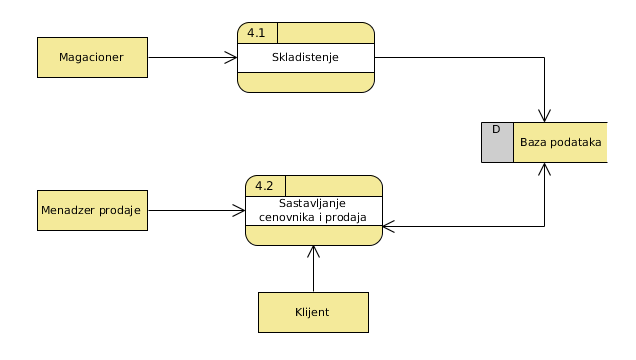
\includegraphics[width=15cm,height=15cm,keepaspectratio]{slike/DTPMagacioniranje.png}\\
			\caption{Dijagram magacioniranja i prodaje}
		\end{figure}
	
	\subsubsection{Sluchaj upotrebe - Skladishtenje}
		
		\begin{itemize}
			\item\textit{Kratak opis} - Artikli koji su stigli do magacina se skladishte u magacin.
			
			\item\textit{Akter} - Magacioner - smeshta artikle u magacin.

			
			\item\textit{Preduslov} - Artikli koji se skladishte su uspeshno dostavljeni do magacina.

			
			\item\textit{Postuslov} - U magacinu se nalaze dostavljeni artikli i u sistemu su isti evidentirani.

			
			\item\textit{Osnovni tok}
				\begin{enumerate}
					\item Magacioner prihvata istovarene artikle.

					\item Magacioner svrstava svaki artikal na odgovorajuc1e mesto u magacinu.

					\item Magacioner pristupa delu informacionog sistema zaduzhenog za artikle.

					\item Magacioner upisuje u sistem informacije o svakom artiklu.

					\item Sistem obaveshtava magacionera o uspeshnom dodavanju artikla.

				\end{enumerate} 

		
			\item\textit{Alternativni tok}
				\begin{enumerate}
					\item [5.] Sistem obaveshtava magacionera da zahtev nije uspeshno obradjen.
- Sluchaj upotrebe se nastavlja od koraka 4.

				\end{enumerate}
			
			\item\textit{Dodatne informacije} - U sistem se upisuje ime artikla, id artikla i kolichina.

			
		\end{itemize}
	
	\subsubsection{Sluchaj upotrebe - Sastavljanje cenovnika i prodaja}
	
		\begin{itemize}
			\item\textit{Kratak opis} - Artiklima koji se nalaze u magacinu menad2er prodaje daje pochetnu cenu i oni se stavljaju na aukciju. 
			
			\item\textit{Akteri}
				\begin{enumerate}
					\item Menad2er prodaje - daje pochetnu cenu artiklima u sistemu.
					\item Klijenti - kupuju artikle na aukciji.
				\end{enumerate}

			
			\item\textit{Preduslov} - Artikli su evidentirani u bazi. 
			
			\item\textit{Postuslov} - Ukoliko je artikal prodat, obrisan je iz baze.

			
			\item\textit{Osnovni tok}
			\begin{enumerate}
				\item Menad2er prodaje pristupa delu informacionog sistema za artikle.
				\item Menad2er prodaje upisuje pochetnu cenu svakom artiklu u sistemu.

				\item Menad2er prodaje odredjuje vreme zavrshetka aukcije.

				\item Klijenti uchestvuju u aukciji.

				\item Sistem objavljuje klijenta sa najvec1om ponudom koji kupuje proizvod.
			\end{enumerate} 

			
			\item\textit{Alternativni tok}
			\begin{enumerate}
				\item [5.] Ako nema nijedne ponude. - Sluchaj upotrebe se nastavlja od koraka 3.
			\end{enumerate}
			
		\end{itemize}
	
	%------------------------------------------------------
	
	
\end{document} 